\chapter{Entwicklungsprozess mit Ionic}
\label{Entwicklungsprozess}

\section{Erstellen und Ausführen}

Für die Entwicklung mit Ionic steht eine eigene Kommandozeilenschnittstelle (CLI) bereit. Diese kann über den Node Package Manager npm installiert werden \cite{ionic:cli}. Die Ionic-CLI gibt manche Kommandos, wie zum Beispiel das \texttt{build}-Kommando an die darunterliegende Cordova-CLI weiter \cite{ionic:build}.

Mit Hilfe des \texttt{start}-Kommandos können neue Ionic-Projekte erstellt werden. Folgender Codeausschnitt zeigt, wie mit der Ionic-CLI ein neues Projekt Ionic2-Projekt mit dem Namen myAwesomeApp erstellt werden kann \cite{ionic:cli}.
\begin{codebox}
\begin{lstlisting}[style=typescript]
$ ionic start myAwesomeApp --v2
\end{lstlisting}
\end{codebox}

Ein erstelltes Projekt kann mit Hilfe des \texttt{serve}-Kommandos im Standard-Browser ausgeführt und getestet werden. Es stehen Optionen zur Verfügung, um bei Änderungen die App neu zu transpilieren und den Browser zu aktualisieren oder die App in einem anderen Browser zu starten \cite{ionic:serve}. Der folgende Codeausschnitt zeigt die Verwendung des \texttt{serve}-Kommandos \cite{ionic:cli}:
\begin{codebox}
\begin{lstlisting}[style=typescript]
$ ionic serve
\end{lstlisting}
\end{codebox}

Nic Raboy nennt in einem Blogeintrag zwei Gründe weshalb es nicht ausreicht Ionic Apps mit dem \texttt{serve}-Kommando im Browser zu testen. Einerseits kann nativer Code, zum Beispiel Cordova-Plugins nicht im Browser ausgeführt werden. Dementsprechend können Funktionalitäten, die auf Cordova-Plugins zurückgreifen, im Browser getestet werden. Andererseits dient Ionic zum Erstellen von mobilen Apps, darum sollte man sie auch als solche auf einem entsprechenden Gerät und nicht nur im Browser testen \cite{raboy:serve}. Die Ionic Dokumentation betont dies ebenfalls:
\begin{citeenv}
	``Since we are building a native (or “hybrid”) app, we can (and should!) test it as one.'' \cite{ionic:testing}
\end{citeenv}

Zu diesem Zweck existiert das \texttt{run}-Kommando. Es ermöglicht es dem Entwickler Ionic-Apps für eine spezielle Plattform zu bauen und auf einem angeschlossenen mobilen Gerät auszuführen. Voraussetzung hierfür ist, dass das USB-Debugging auf dem Gerät aktiviert ist. Auch bei diesem Kommando gibt es die Option, die App bei Änderungen automatisch zu aktualisieren \cite{ionic:run}. Um eine Ionic-App auf einem verbundenen Android-Gerät auszuführen, kann das \texttt{run}-Kommando wie folgt genutzt werden:
\begin{codebox}
\begin{lstlisting}[style=typescript]
$ ionic run android
\end{lstlisting}
\end{codebox}

\section{Debugging}

Um eine App zu testen muss sie zuerst, wie im vorhergehenden Abschnitt beschrieben im Browser oder auf einem mobilen Gerät ausgeführt werden. 

Wird die App im Browser des Entwicklungsrechners ausgeführt, erfolgt das Debugging entsprechend einer normalen Webapplikation: Über die Entwicklertools des Browsers können Elemente inspiziert, die Logs der JavaScript-Konsole eingesehen oder Haltepunkte gesetzt werden \cite{ionic:tips}. Eine ausführliche Beschreibung der Entwicklertools pro Browser würde an dieser Stelle zu weit führen und ist beispielsweise in \cite{google:chrome} für Chrome oder \cite{apple:safari} für Safari zu finden.

Für das Debugging der App auf einem mobilen Gerät ist etwas mehr Vorbereitung nötig. Im folgenden sollen die notwendigen Schritte angesprochen werden, um mit Chrome eine App auf einem angeschlossenen Android-Gerät zu untersuchen.

Dazu muss die Android Debug Bridge (adb) installiert werden \cite{ionic:tips}. Dabei handelt es sich um ein Tool aus dem Android Software Development Kit, dass die Kommunikation zwischen dem Entwicklungsrechner und angeschlossenen Geräten vereinfacht. Die adb kann über die Kommandozeile angesprochen werden und ermöglicht beispielsweise das Installieren von Apps \cite{google:adb}. Mit Hilfe des folgenden Kommandos werden alle verbundenen Geräte aufgelistet und somit sichergestellt, dass ein verbundenes Gerät von der adb erkannt wurde \cite{ionic:tips}:
\begin{codebox}
\begin{lstlisting}[style=typescript]
$ adb devices
\end{lstlisting}
\end{codebox}

Wird die zu untersuchende App nun auf dem verbundenen Gerät ausgeführt, so erscheint das Gerät und die App in Chrome unter der URL \texttt{chrome://inspect/\#devices}, wie in Abbildung \ref{fig:inspect} ersichtlich \cite{ionic:tips}.

\begin{figure}[htb]
	\centering
	\caption{\texttt{Chrome://inspect} mit einem verbundenem Gerät (GT-I9195) und gestarteter App (ionicpouch)}
	\label{fig:inspect}
	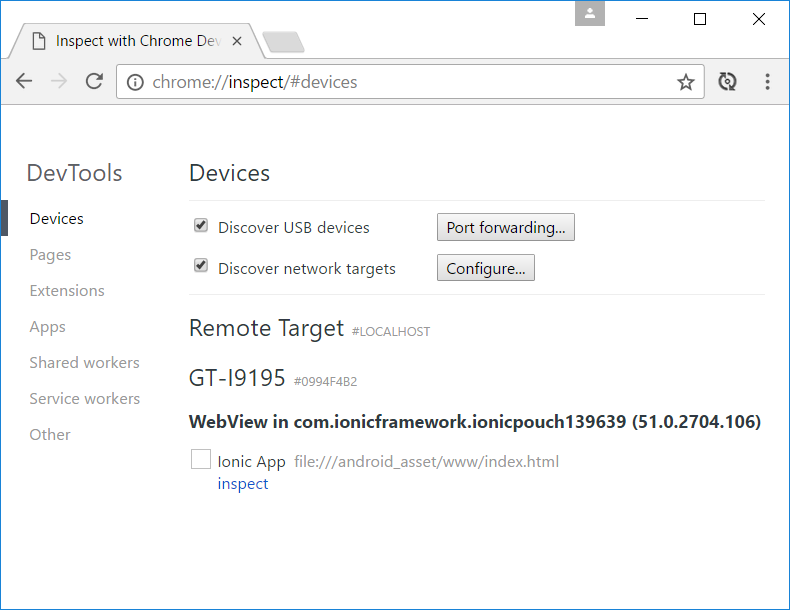
\includegraphics[width=\textwidth]{\figdir/chrome-inspect.png}
\end{figure}

Durch den \texttt{inspect}-Link in Abbildung \ref{fig:inspect} kann die App nun, wie bereits beschrieben im Browser untersucht werden \cite{ionic:tips}.

